
\documentclass[12pt,epsfig,color,russian]{article}
\usepackage[russian]{babel}
\usepackage{epsfig}
\usepackage{color}

\topmargin=0cm
\hoffset -30mm
\voffset -12mm
\setlength{\unitlength}{1mm}
\parindent=10mm
\textheight=250mm
\textwidth=185mm
\pagestyle{empty}

\begin{document}
\sf\Large

Как МАКРО-параметры ($R,T,p,...$) связать с МИКРО-параметрами $(v,E_k,...$)? Если бы знать число Авогадро $N$ или число Лошмидта $n_0$ или постоянную Больцмана $k$ -- только КАК их измерить?

Достаточно мелкие МАКРО-объекты (броуновские частицы) в окру\-же\-нии молекул должны быть с ними в тепловом равновесии $\Rightarrow$ их средняя кинетическая энергия $W$ равна кинетической энергии молекул $w$ при дан\-ной $T$:\vspace{-3mm}
\begin{displaymath}
\overline{W}=\overline{w}=\frac32\;kT = \frac32\cdot\frac RN\cdot T
\end{displaymath}
Их видно в микроскоп $\Rightarrow$ можно попытаться определить $\overline{W}$. Из-за хао\-тич\-но\-с\-ти движения $\overline{v^2}$ измерить напрямую не удается.\\
\begin{picture}(190,110)(0,0)
 %\put(0,0){\framebox(190,100)[b]{}}
 \put(0,0){\includegraphics{GP010F01.eps}}
 \put(40,104){\makebox(0,0)[tl]{\parbox{150mm}{
Жан Батист Перрен (J.B.Perrin, 1870-1942, Lille) использовал барометрическую формулу:
\begin{displaymath}
n_h=n_0\cdot\exp\left(-\frac{Mgh}{kT}\right)=
n_0\cdot\exp\left(-\frac{3Mgh}{2\overline{W}}\right).
\end{displaymath}
Подсчитывая через микроскоп число частиц $n_h$ в слоях на разной высоте с шагом в несколько микрон, он определил показатель экспоненты и нашел затем $\overline{W}$:
\begin{displaymath}
\overline{W}=\frac{3Mg(h_2-h_1)}{2\ln\left(\frac{n_1}{n_2}\right)}
\end{displaymath}
Радиус частиц определялся из формулы Стокса по скорости оседании ``мути'', а из радиуса находился вес $Mg$. В итоге Перрен получил (1909 г.), что $N\simeq6\cdot10^{23}$ 1/моль.
 }}}
\end{picture}
\begin{picture}(190,60)(0,0)
 %\put(0,0){\framebox(190,60)[b]{}}
 \put(110,0){\includegraphics{GP010F02.eps}}
 \put(0,55){\makebox(0,0)[tl]{\parbox{140mm}{
Второй метод Перрена: измерение среднего смещения частицы $\overline{x^2}$ за время $t$ и затем использование формулы Эйнштейна-Смолуховского:
\begin{displaymath}
\overline{x^2}=\frac{RT}{3\pi\eta N}\cdot t
\end{displaymath}
где $\eta$ -- вязкость жидкости. Результат получился тот же.\\
В итоге (1926 г.) -- {\color{red}\bf Нобелевская премия!}
 }}}
\end{picture}\\
\voffset -25mm
\underline{\bf Длина свободного пробега молекулы} -- среднее расстояние между двумя столкновениями.\\
\begin{picture}(190,47)(0,0)
 %\put(0,0){\framebox(190,50)[b]{}}
 \put(77,0){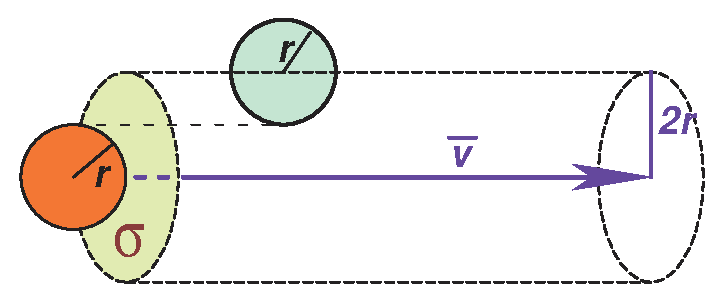
\includegraphics{GP010F03.eps}}
 \put(0,0){\makebox(0,0)[bl]{\parbox{75mm}{
Молекула задевает другие мо\-ле\-ку\-лы, если их центры лежат внутри цилиндра с радиусом $2r$ и площадью основания $\sigma=\pi(2r)^2$. Принято говорить, что она обладает {\bf сечением} ${\bf \sigma}$.
 }}}
\end{picture}\\
за 1 секунду она заденет все, что находится внутри цилиндра длиной $\overline{v}$, то есть, число столкновений молекулы в единицу времени\vspace{-2mm}
\begin{displaymath}
n=\sigma\;\overline{v}\sqrt{2}\;n_0=4\sqrt{2}\;\pi\;r^2\;\overline{v}\;n_0
\vspace{-2mm}
\end{displaymath}
($\sqrt{2}$ добавился потому, что на самом деле вместо средней скорости $\overline{v}$ должна быть средняя {\bf встречная} скорость молекул; можно показать, что она в $\sqrt{2}$ раз больше). Прикинем порядок $n$:
\begin{displaymath}
n\sim4\cdot1.4\cdot3.14\cdot10^{-16}\texttt{см}^2\cdot5\times10^4\texttt{см/с }\cdot3\times10^{19}\texttt{см}^{-3}\simeq3\times10^9\texttt{1/с}
\end{displaymath}
То есть, при н.у. каждая молекула сталкивается с частотой 3 ГГц. Свободный пробег при этом равен
\begin{displaymath}
\lambda=\frac{\overline{v}}{n}=\frac1{\sqrt{2}\;\sigma\;n_0}\simeq
\frac{5\times10^4\texttt{ см/с}}{3\times10^9\texttt{ 1/с}}\simeq10^{-5}\texttt{ см}=0.1\texttt{ мкм}
\end{displaymath}
Как видим, $\lambda$ зависит от молекулярной плотности газа (от числа молекул в 1 см$^3$) и от размеров молекул (от сечения $\sigma$), но не от скорости (и связанной с нею температуры)! В действительности это не совсем так:
\begin{displaymath}
\lambda=\lambda_\infty\;\frac{T}{C+T}
\end{displaymath}
Где $C$ -- постоянная Сезерлэнда. Для азота, например, $C=102.7 K$.

Каков свободный пробег молекул азота при разных давлениях?
\begin{center}
\begin{tabular}{|c||p{22mm}|p{22mm}|p{22mm}|p{22mm}|}\hline
Давление [мм рт.ст.] & 760  & 1  & $10^{-3}$ & $10^{-6}$ \\ \hline \hline
Пробег $\lambda$ & 0.07 мкм & 50 мкм & 5 см & 50 м\\ \hline
\end{tabular}
\end{center}
{\bf Вакуум} -- состояние вещества (газа), при котором длина свободного пробега больше размеров сосуда: $\lambda\gg L$. Молекулы не сталкиваются, а просто летают от стенки до стенки (или сидят на них).
\newpage
\underline{\bf Опыты с молекулярными пучками}\\

{\bf Опыт Штерна}: при вращении двойного цилиндра с угловой скоростью $\omega$ след от молекулярного пучка отстает на дугу $s$:\\
\begin{picture}(190,85)(0,0)
 %\put(0,0){\framebox(190,85)[b]{}}
 \put(0,0){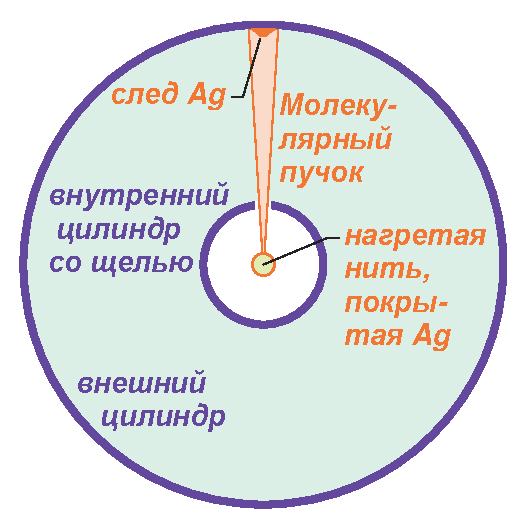
\includegraphics{GP010F04.eps}}
 \put(100,0){\includegraphics{GP010F05.eps}}
\end{picture}\\
Время пролета молекул от щели до внешнего цилиндра: $t=R/\overline{v}$.
За это время цилиндр поворачивается на некий угол, и дуга равна
\begin{displaymath}
s=\omega Rt\hspace{20mm}\Rightarrow\hspace{20mm}t=s/\omega R
\end{displaymath}
Приравнивая $t$, получим уравнение, из него найдем скорость молекул:
\begin{displaymath}
\frac{s}{\omega R}=\frac{R}{\overline{v}}\hspace{20mm}\Rightarrow\hspace{20mm}\overline{v}=\frac{\omega R^2}s
\end{displaymath}
\\[5mm]
{\bf Вариант опыта Штерна :}\\
\begin{picture}(190,60)(0,0)
 %\put(0,0){\framebox(190,60)[b]{}}
 \put(10,0){\includegraphics{GP010F06.eps}}
\end{picture}\\
\textheight=260mm
\underline{\bf Явления переноса} -- теплопроводность, внутреннее трение, диффузия.\\

{\bf Диффузия.} Если $\overline{v}\simeq$500 м/с, то почему запахи распространяются ме\-д\-лен\-но? Ответ: потому что $\lambda\simeq$0.1 мкм. Молекулы толкутся, хоть и очень бы\-с\-т\-ро, но на месте!

\noindent
\begin{picture}(190,90)(0,0)
 %\put(0,0){\framebox(190,90)[b]{}}
 \put(0,0){\includegraphics{GP010F07.eps}}
 \put(60,0){\includegraphics{GP010F08.eps}}
 \put(80,90){\makebox(0,0)[tl]{\parbox{105mm}{
МАКРОскопический опыт показывает, что масса газа $\Delta M$, диффундирующая через площадку $\Delta S$ за время $\Delta t$ про\-пор\-ци\-о\-наль\-на площадке $\Delta S$, времени $\Delta t$ и градиенту плотности газа $(\rho_1-\rho_2)/\Delta x$:
 }}}
 \put(185,55){\makebox(0,0)[tr]{\parbox{60mm}{
\begin{displaymath}
\Delta M\sim \Delta S\cdot\Delta t\cdot\left(\frac{\Delta\rho}{\Delta x}\right)
\end{displaymath}
или, в термнах потока:
\begin{equation}
\vec{\Phi}(M)=-D \vec{\nabla}\rho
\end{equation}
где $\vec{\nabla}\rho\equiv(\frac{\partial\rho}{\partial x},\frac{\partial\rho}{\partial y},\frac{\partial\rho}{\partial z})$,
}}}
\end{picture}\\
$D$ -- коэффициент диффузии, а знак ``$-$'' символизирует то, что поток распространяется в направлении УМЕНЬШЕНИЯ, а не УВЕЛИЧЕНИЯ плотности газа $\rho$.\\

\noindent
\begin{picture}(190,40)(0,0)
 %\put(0,0){\framebox(190,50)[b]{}}
 \put(100,0){\includegraphics{GP010F09.eps}}
 \put(0,43){\makebox(0,0)[tl]{\parbox{95mm}{
Теперь рассмотрим то же самое яв\-ле\-ние с точки зрения молекул. Пусть $\exists$ 2 похожих газа {\bf A} и {\bf B}, взаимно диффундирующих навстречу друг другу. Выделим два кубика с ребром $L$ и такую же площадку $\Delta S=$
}}}
\end{picture}\\
$=L^2$ между ними, причем дистанцию выберем равной длине свободного пробега $\lambda$. Пусть концентрация молекул {\bf A} и {\bf B} в 1 см$^3$ составляет $n_A$ и $n_B$, соответственно. Тогда в первом кубике содержится $n_AL^3$, а во втором -- $n_BL^3$ молекул. Пространство однородно и изотропно $\Rightarrow$ 1/3 движется вдоль $x$, 1/3 вдоль $y$ и 1/3 вдоль $z$. Из 1/3 половина -- направо и половина -- налево. $\Rightarrow$ из кубика A направо летит $n_AL^3/6$ молекул, а из кубика B $n_BL^3/6$ молекул летит налево. Т.к. до площадки $\Delta S$ расстояние =$\lambda$, то все они эту площадку пересекут за время $\delta t=L/\overline{v}$ (разница между первыми и последними молекулами из одного кубика). Итак, за единицу времени через площадку  $\Delta S$ направо пролетает число A-молекул:
\begin{displaymath}
n_\rightarrow = \frac{n_A\cdot L^3}{6\cdot\delta t}=\frac{n_A\cdot L^3\cdot\overline{v}}{6\cdot L}=
\frac{n_A\cdot L^2\cdot\overline{v}}{6}
\end{displaymath}
Аналогично, налево пролетает
\begin{displaymath}
n_\leftarrow = \frac{n_B\cdot L^2\cdot\overline{v}}{6}
\end{displaymath}
Итоговый транзит молекул через площадку $\Delta S$ составляет
\begin{displaymath}
\Delta n=(n_\rightarrow-n_\leftarrow) =
\frac{\left(n_A-n_B\right)\cdot L^2\cdot\overline{v}}{6}
\end{displaymath}
За произвольный промежуток времени $\Delta t$ это количество будет в $\Delta t$ раз больше, а переносимая масса составит
\begin{displaymath}
\Delta M=m\cdot\Delta n\cdot\Delta t=
\frac{m\cdot \left(n_A-n_B\right)\cdot L^2\cdot\overline{v}\cdot\Delta t}{6}
\end{displaymath}
Каков градиент плотности газа?
\begin{displaymath}
\frac{\Delta\rho}{\Delta x}=\frac{m\cdot \left(n_B-n_A\right)}{2\lambda}
\end{displaymath}
C учетом этого, получаем:
\begin{displaymath}
\Delta M=-\frac13\;\lambda\;\overline{v}\;\left(\frac{\Delta\rho}{\Delta x}\right)\;\Delta t\;\Delta S
\end{displaymath}
Сравнивая это с полученным в МАКРО-опыте, находим:
\begin{displaymath}
D=\frac{\lambda\;\overline{v}}3
\end{displaymath}
Имеем в виду, что $\overline{v}=\sqrt{8kT/\pi m}$, а $\lambda=1/\sqrt{2}\sigma n_0$, и делаем выводы:
\begin{itemize}
\item $D\sim \sqrt{T}$
\item $D\sim 1/\sqrt{\mu}$
\item $D\sim 1/p$
\item $D\sim 1/\sigma$
\end{itemize}
{\bf Теплопроводность.} Тут дело несколько осложняется {\bf конвекцией}. Что\-бы от нее избавиться, надо измерения проводить по вертикали, причем сверху $T$ > чем снизу.

МАКРОскопический опыт показывает, что количество тепла $\Delta Q$, пе\-ре\-но\-симое через площадку $\Delta S$ за время $\Delta t$ про\-пор\-ци\-о\-наль\-но площадке $\Delta S$, времени $\Delta t$ и градиенту температуры газа $(T_1-T_2)/\Delta x$:\vspace{-2mm}
\begin{displaymath}
\Delta Q=- \chi\Delta S\cdot\Delta t\cdot\left(\frac{\Delta T}{\Delta x}\right)
\hspace{10mm}\texttt{или, в терминах потока:}\hspace{5mm}\vec{\Phi}(Q)=-\chi \vec{\nabla}T
\end{displaymath}
где $\vec{\nabla}T\equiv(\frac{\partial T}{\partial x},\frac{\partial T}{\partial y},\frac{\partial T}{\partial z})$,
$\chi$ -- коэффициент теплопроводности, а знак ``$-$'' символизирует то, что поток распространяется в направлении УМЕНЬ\-ШЕ\-НИЯ, а не УВЕЛИЧЕНИЯ  температуры $T$.

Теперь снова рассмотрим то же самое явление с точки зрения молекул. Опять те же 2 кубика, только не с разными газами, а с разной температурой. Тут в качестве переносимого объекта выступает энергия молекулы $w=\frac12ikT$, где $i$ -- число степеней свободы. Повторив все выкладки, получим, что направо переносится\vspace{-5mm}
\begin{displaymath}
Q_\rightarrow =
\frac16\cdot n_A\cdot \Delta S\cdot \Delta t\cdot\overline{v_A}\cdot\frac i2kT_A
\end{displaymath}
а налево -- \vspace{-3mm}
\begin{displaymath}
Q_\leftarrow =
\frac16\cdot n_B\cdot \Delta S\cdot \Delta t\cdot\overline{v_B}\cdot\frac i2kT_B
\end{displaymath}
В итоге, перенос тепла составит\vspace{-3mm}
\begin{displaymath}
\Delta Q=Q_\rightarrow-Q_\leftarrow =
\frac16\cdot\frac i2k \cdot\left(n_A\cdot\overline{v_A}\cdot T_A - n_B\cdot\overline{v_B}\cdot T_B \right) \Delta S\cdot \Delta t
\end{displaymath}
Поскольку $n\sim\frac1T$, а $\overline{v}\sim\sqrt{T}$, то их произведение $nv\sim1/\sqrt{T}$ -- от $T$ зависит слабо, и в первом приближении этой зависимостью можно пренебречь. Тогда\vspace{-3mm}
\begin{displaymath}
\Delta Q=
\frac16\cdot\frac i2k \cdot n_0\cdot\overline{v}\cdot \left(T_A - T_B \right) \Delta S\cdot \Delta t=-\frac13\cdot n_0\cdot\overline{v}\cdot\lambda\cdot\frac i2k \cdot \left(\frac{\Delta T}{\Delta x} \right)\Delta S\cdot \Delta t
\end{displaymath}
и коэффициент теплопроводности $\chi$ равен
\begin{displaymath}
\chi=\frac13\cdot n_0\cdot\overline{v}\cdot\lambda\cdot\frac i2k =
\frac13\;\frac{n_0}N\cdot\overline{v}\cdot\lambda\cdot C_V=
\frac13\;\rho\cdot\overline{v}\cdot\lambda\cdot c_V
\end{displaymath}
(с учетом того, что $k=R/N$, $n_0/N=\rho/\mu$, а теплоемкость $C_V=iR/2$)
\newpage
\noindent
{\bf Внутреннее трение.} Аналогично жидкостям: слой, который движется \\
\begin{picture}(190,102)(0,0)
 %\put(0,0){\framebox(190,100)[b]{}}
 \put(0,0){\includegraphics{GP010F10.eps}}
 \put(20,100){\makebox(0,0)[tl]{быстрее, тащит за собою более медленные слои, а те его тормозят.}}
 \put(40,87){\makebox(0,0)[tl]{\parbox{150mm}{
Схема опыта по измерению внутреннего трения в газе. Внешний цилиндр висит на упругой струне, а внутренний вращается со скоростью $\omega$ (при этом, линейная скорость поверхности внутреннего цилиндра $\omega R$=$u$). Через слои газа вращающий момент передается на внешний цилиндр и закручивает струну. Измерив закручивающий момент, можно найти величину $f$ силы внутреннего трения в газе, действующую по касательной к каждой маленькой площадке $\Delta S$:
\begin{displaymath}
f=\eta\left(\frac{\Delta u}{\Delta r}\right)\Delta S
\end{displaymath}
С точки зрения молекулярно-кинетической теории, к слу-
 }}}
\end{picture}\\
\begin{picture}(190,39)(0,0)
 %\put(0,0){\framebox(190,40)[b]{}}
 \put(115,0){\includegraphics{GP010F11.eps}}
 \put(0,36){\makebox(0,0)[tl]{\parbox{110mm}{
чайным скоростям молекул $\vec{v}$ в каждом слое газа добавляется переносная скорость $\vec{u}$, постоянная для данного слоя. Попадая в соседний слой, каждая молекула приносит туда дополнительный импульс $m\vec{u}$ и таким
 }}}
\end{picture}\\
образом ускоряет или замедляет этот слой. Рассмотрим площадку $\Delta S$ и два слоя газа {\bf \color{red}A} и {\bf \color{blue}B}, отстоящие от нее на расстояние пробега $\lambda$ и движущиеся со скоростями $u_A$ и $u_B$, соответственно. Как мы уже видели выше, число молекул, попадающих за время $\Delta t$ из одного слоя в другой, равно\vspace{-5mm}
\begin{displaymath}
n_\uparrow=n_\downarrow=\frac16\cdot n_0\cdot\overline{v}\cdot\Delta S\cdot\Delta t
\end{displaymath}
Количество движения (импульс), переносимое этими молекулами из слоя в слой, равно\vspace{-6mm}
\begin{displaymath}
K_{\uparrow,\downarrow}=n_{\uparrow,\downarrow}\cdot mu_{A,B}=m\cdot u_{A,B}\cdot\frac16\cdot n_0\cdot\overline{v}\cdot\Delta S\cdot\Delta t
\end{displaymath}
В итоге, импульс, передаваемый от слоя {\bf \color{red}A} к слою  {\bf \color{blue}B}, составит
\begin{displaymath}
\Delta K =K_{\uparrow}-K_\downarrow=
\frac16\cdot m\cdot n_0\cdot\overline{v}\cdot (u_A-u_B)\cdot\Delta S\cdot\Delta t
\end{displaymath}
Так как $m\cdot n_0$ -- это плотность газа $\rho$, а $(u_A-u_B)/2\lambda$ -- это градиент скорости $\Delta u/\Delta z$, то
\begin{displaymath}
\Delta K =
\frac13\cdot\rho\cdot\overline{v}\cdot\lambda\left(\frac{\Delta u}{\Delta z}\right)\cdot\Delta S\cdot\Delta t
\end{displaymath}
и коэффициент трения газа равен
\begin{equation}\label{Eq.eta}
\eta=\frac13\cdot\rho\cdot\overline{v}\cdot\lambda\hspace{10mm}
\end{equation}
Сравните с коэффициентом теплопроводности:
\begin{equation}\label{Eq.chi}
\chi=\frac13\cdot\rho\cdot\overline{v}\cdot\lambda\cdot c_V
\end{equation}
Здесь скорость молекул $\overline{v}$ от давления не зависит, плотность $\rho\sim p$, а пробег $\lambda\sim1/p$. Таким образом, и трение $\eta$, и теплопроводность $\chi$ от давления зависеть не должны. Странный вывод... Однако, в действитель\-но\-с\-ти так и есть (в таблице -- данные по трению в CO$_2$):
\begin{center}
\begin{tabular}{|c||p{25mm}|p{25mm}|p{25mm}|p{25mm}|p{25mm}|}\hline
$p$ [мм рт.ст.] & 760  & 380  & 20 & 2 & 0.6 \\ \hline \hline
$\eta$ [г/см/с] &
$14.9\cdot10^{-5}$&
$14.9\cdot10^{-5}$&
$14.8\cdot10^{-5}$&
$14.7\cdot10^{-5}$&
$13.8\cdot10^{-5}$ \\ \hline
\end{tabular}
\end{center}
Но при очень низких давлениях зависимость трения $\eta$ и теплопроводности $\chi$ от давления появляется (они начинают падать)! \\
\begin{picture}(190,110)(0,0)
 %\put(0,0){\framebox(190,110)[b]{}}
 \put(20,60){\includegraphics{GP010F12.eps}}
 \put(140,0){\includegraphics{GP010F13.eps}}
 \put(0,50){\makebox(0,0)[tl]{\parbox{130mm}{
Причина: пробег $\lambda$ становится больше размеров $L$ измерительного устройства $\Rightarrow$ при этих условиях в формулах (\ref{Eq.eta}) и (\ref{Eq.chi}) надо заменить $\lambda\rightarrow L$, и тогда $\eta$ и  $\chi$ становятся про\-пор\-ци\-о\-наль\-ны\-ми плотности $\rho$ и $\Rightarrow$ давлению $p$. Применение: сосуд Дьюара (1892). James Dewar, 1842-1923, Эдинбург. Производство: Termos GmbH, Германия, 1904.
 }}}
\end{picture}\\
\newpage
{\bf Устройства для получения и измерения низких давлений.}\\

Механические \underline{форвакуумные насосы}: {\sl поршневые}, {\sl роторные}, {\sl диа\-фраг\-мен\-ные} --
для получения ``форвакуума'' ($10^{-2}\ldots10^{-3}$ мбар)\\
\begin{picture}(190,72)(0,0)
 %\put(0,0){\framebox(190,70)[b]{}}
 \put(5,0){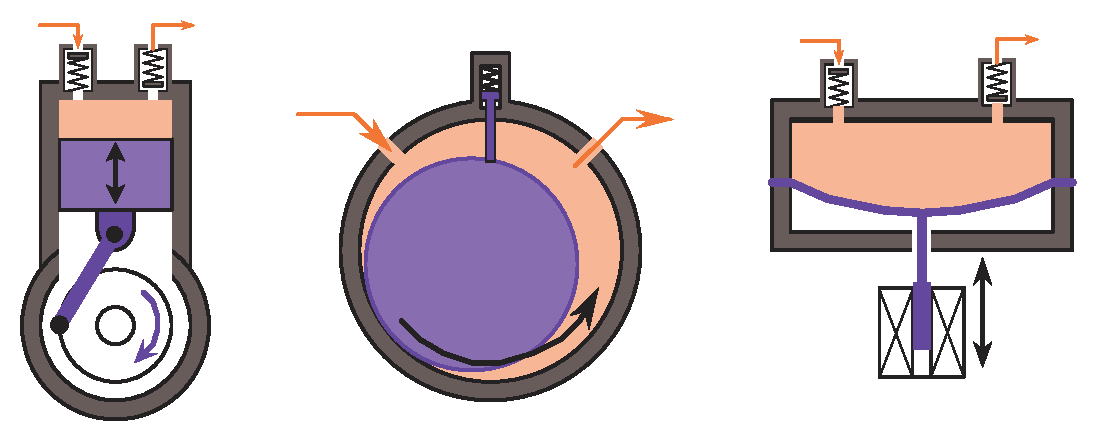
\includegraphics{GP010F14.eps}}
\end{picture}\\

\underline{Высоко-вакуумные насосы:}
\begin{itemize}
\item {\sl диффузионные (паромасляные)} --- Масло нагревается и испаряется, а затем снова конденсируется, прихватывая с собой молекулы оста\-то\-ч\-но\-го газа.\\
    {\color{blue}(+) простота и большая производительность}\\
    {\color{red}(---) пары масла попадают в откачиваемый объем}
\item {\sl магниторазрядные} --- титановый электрод распыляется в электри\-че\-с\-ком поле; ускоренные ионы титана, вбиваясь затем в поверхность, тащат за собой молекулы газа. Магнитное поле -- для увеличения пути ионов в откачиваемом объеме.\\
    {\color{blue}(+) чистый вакуум, нет вибраций}\\
    {\color{red}(---) малые ресурс и производительность}
\item {\sl турбо-молекулярные} --- быстро вращающийся вентилятор (турбина).\\
    {\color{blue}(+) чистый вакуум}\\
    {\color{red}(---) высокая стоимость}
\item {\sl криогенные} --- остаточный газ вымораживается на твердой поверхности.\\
    {\color{blue}(+) очень чистый вакуум}\\
    {\color{red}(---) малая производительность; гелий и водород не замерзают}
\end{itemize}
\newpage
\underline{Вакуумметры}
\begin{itemize}
\item {\sl механические (классические) анероиды}\\
 \begin{picture}(170,40)(0,0)
 %\put(0,0){\framebox(175,40)[b]{}}
 \put(135,0){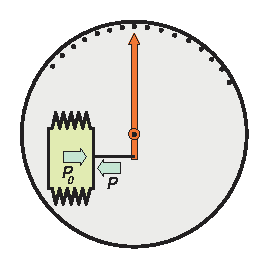
\includegraphics{GP008F02.eps}}
 \put(0,35){\makebox(0,0)[tl]{\parbox{130mm}{
--- механическое расширение/сжатие гермообъема с газом под действием измеряемого давления\\
    {\color{blue}(+) простота}\\
    {\color{red}(---) грубая шкала; диапазон от 1 ат. до 10 мбар}
 }}}
 \end{picture}
\item {\sl пьезоэлектрические или емкостные анероиды}\\
--- то же самое, но измерение величины сжатия -- более точное\\
    {\color{blue}(+) простота}\\
    {\color{red}(---) грубая шкала; диапазон от 1 ат. до 1 мбар}
\item {\sl жидкостные (ртутные)}\\
 \begin{picture}(170,45)(0,0)
 %\put(0,0){\framebox(175,45)[b]{}}
 \put(160,0){\includegraphics{GP008F03.eps}}
 \put(0,40){\makebox(0,0)[tl]{\parbox{155mm}{
--- измерение перепада уровня жидкости под действием измеряемого давления\\
    {\color{blue}(+) простота}\\
    {\color{red}(---) грубая шкала; диапазон от 1 ат. до 1 мбар; опасность попадания паров жидкости в измеряемый объем}
 }}}
 \end{picture}
\item {\sl термопарные}\\
 \begin{picture}(170,25)(0,0)
 %\put(0,0){\framebox(175,35)[b]{}}
 \put(120,-10){\includegraphics{GP010F15.eps}}
 \put(0,20){\makebox(0,0)[tl]{\parbox{125mm}{
--- измерение теплопроводности газа\\
    {\color{blue}(+) простота, надежность, безопасность}\\
    {\color{red}(---) форвакуумный диапазон $10\ldots10^{-3}$ мбар}
 }}}
 \end{picture}
\item {\sl ионизационные}\\
--- ионизация остаточного газа и измерение ионного тока\\
    {\color{blue}(+) высоковакуумный диапазон $10^{-3}\ldots10^{-10}$ мбар}\\
    {\color{red}(---) ненадежность, малый ресурс}
\item {\sl комбинированные}\\
--- термопарные + на эффекте Пеннинга (ионизация с холодным катодом)\\
    {\color{blue}(+) высокая надежность, широкий диапазон $10\ldots10^{-10}$ мбар}\\
    {\color{red}(---) высокая стоимость, малый ресурс}
\end{itemize}


\end{document}
